\chapter{Progettazione concettuale}

\section{Utenti standard}

\subsection{Gestione pubblicazione ricette}

\begin{figure}[H]
    \centering
    % Regola la larghezza. 0.8\textwidth significa "80% della larghezza del testo".
    % Puoi usare anche cm, es: width=10cm
    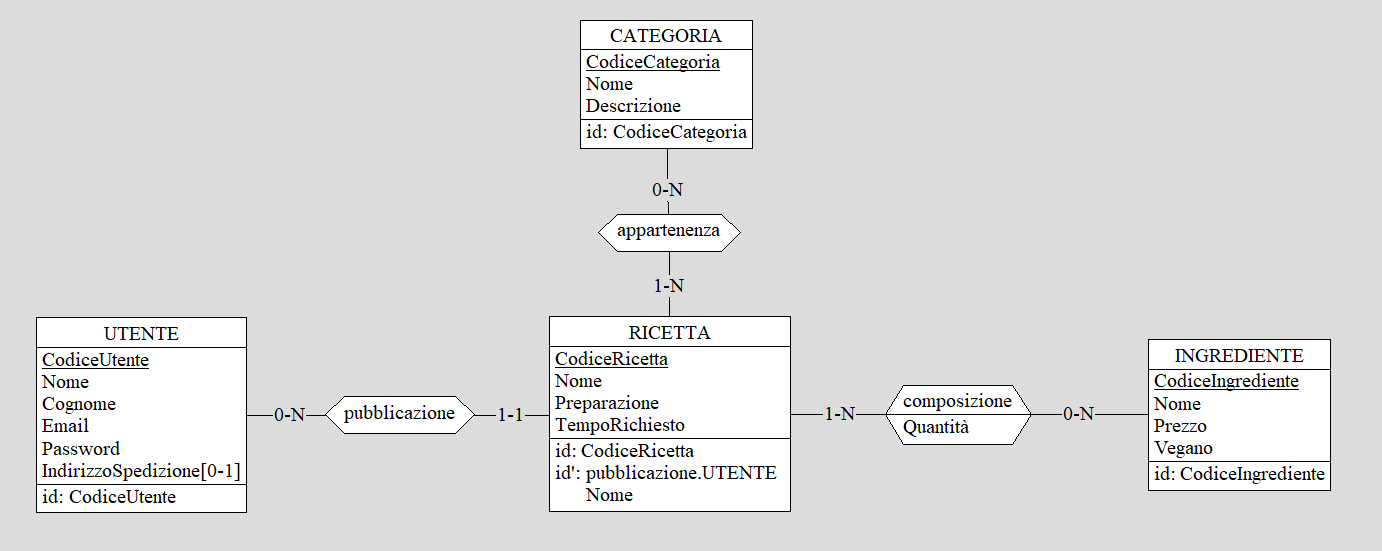
\includegraphics[width=1\textwidth]{images/conc_pubblicazione.png}
    \caption{Schema scheletro per la pubblicazione ricette}
    \label{fig:pubbl} % Etichetta per fare riferimento: vedi Figura \ref{fig:mia_immagine}
\end{figure}


Secondo il nostro dominio, un \textbf{utente} al momento della registrazione deve inserire obbligatoriamente le sue generalità e opzionalmente un indirizzo di spedizione. L’\textbf{utente} quindi rappresenta un’entità fondamentale nel nostro schema concettuale, ed è identificato da un codice univoco (CodiceUtente) assegnato dal sistema in maniera progressiva e automatica al momento della registrazione. Si è deciso di non usare il codice fiscale come identificatore per due motivi principali: 
\begin{itemize}
    \item La maggior parte dei ricettari online non richiede il codice fiscale dell'utente.
    \item Evitare casi estremi di coincidenza di codici fiscali.
\end{itemize}

Un \textbf{utente}, una volta registrato al sito, può pubblicare delle \textbf{ricette},  le quali posseggono un codice univoco progressivo (CodiceRicetta) e un identificatore alternativo (Utente, nomeRicetta) e sono associate a un solo \textbf{utente}, ovvero colui che la pubblica.

Si è deciso in fase di progettazione concettuale di tenere valida la chiave primaria CodiceRicetta, in quanto la chiave alternativa composta (Utente, NomeRicetta) avrebbe portato al pericolo di ridondanze e complicazioni per quanto riguarda un futuro aggiornamento del Database e la sua effettiva propagazione. 
\\L’identificatore alternativo (Utente, nomeRicetta) verrà successivamente espresso come vincolo UNIQUE in fase di progettazione logica, in modo tale da modellare correttamente il vincolo di dominio secondo il quale un \textbf{utente} non può pubblicare ricette omonime.

Al momento della pubblicazione della \textbf{ricetta}, oltre agli attributi generali bisogna associarvi obbligatoriamente almeno un \textbf{ingrediente}, indicando anche la sua relativa quantità, la quale viene salvata nell’associazione \textbf{composizione} come attributo. \\
Dopo aver aggiunto almeno un \textbf{ingrediente} va aggiunta obbligatoriamente almeno una \textbf{categoria} di appartenenza per la \textbf{ricetta}, la quale è identificata da un codice univoco (CodiceCategoria). \\
Gli ingredienti sono identificati da un codice univoco (CodiceIngrediente), in più dispongono di un nome, un prezzo €/Kg e un attributo booleano (Vegano) che chiarisce se un determinato \textbf{ingrediente} sia derivato da animali o meno.

\subsection{Gestione recensioni}

\begin{figure}[H]
    \centering
    % Regola la larghezza. 0.8\textwidth significa "80% della larghezza del testo".
    % Puoi usare anche cm, es: width=10cm
    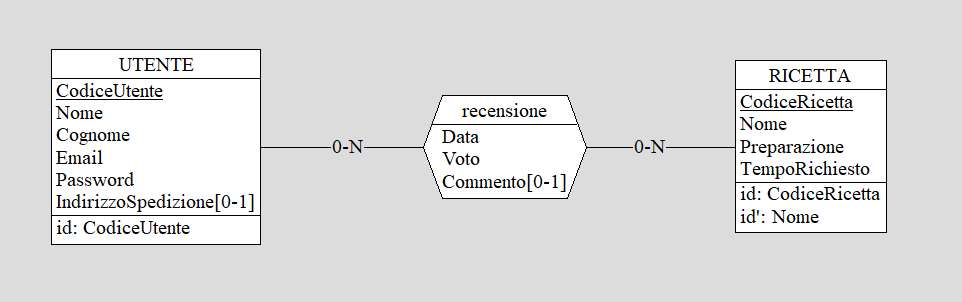
\includegraphics[width=1\textwidth]{images/conc_recensione.png}
    \caption{Schema scheletro per la recensione di ricette}
    \label{fig:recens} % Etichetta per fare riferimento: vedi Figura \ref{fig:mia_immagine}
\end{figure}


Secondo le regole di dominio, un \textbf{utente} può lasciare più recensioni a \textbf{ricette} diverse (non più di una recensione per una stessa ricetta) e una \textbf{ricetta} può avere più \textbf{recensioni} da parte di più \textbf{utenti}.


Inizialmente si era pensato di reificare l’associazione \textbf{recensione} in una entità, ma progredendo nello sviluppo ci si è resi conto che questa entità era composta esclusivamente da identificatori esterni (una recensione poteva essere identificata solamente tramite utente e ricetta a cui era associata), quindi si è optato per renderla un’associazione, in quanto non possono esistere due tuple che abbiano stessi \textbf{utente} e \textbf{ricetta}.

 
L’associazione \textbf{recensione} prevede alcuni attributi obbligatori, come Data e Voto, e un attributo opzionale, ovvero il commento.
Tutto ciò rappresenta come funziona al giorno d’oggi il sistema delle recensioni in approssimativamente tutti i casi.

\subsection{Gestione ordini}

\begin{figure}[H]
    \centering
    % Regola la larghezza. 0.8\textwidth significa "80% della larghezza del testo".
    % Puoi usare anche cm, es: width=10cm
    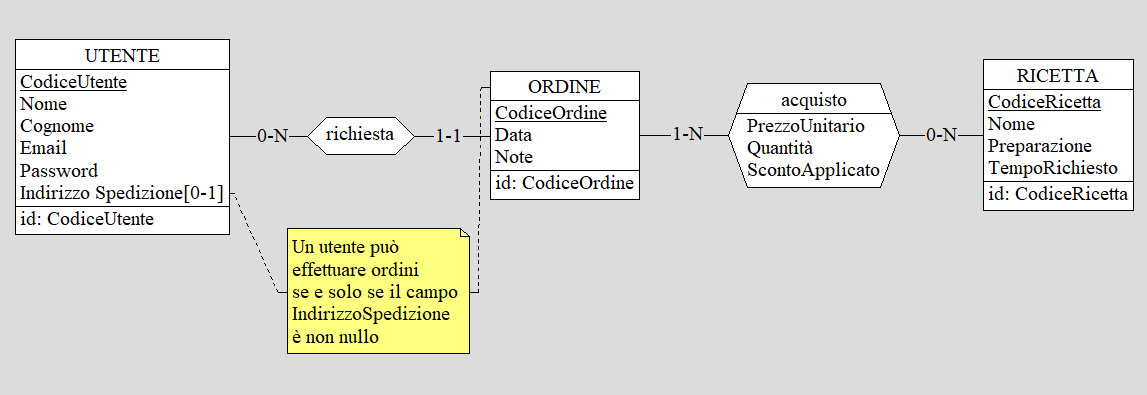
\includegraphics[width=1\textwidth]{images/conc_ordine.png}
    \caption{Schema scheletro per l'ordine di ricette.}
    \label{fig:ord} % Etichetta per fare riferimento: vedi Figura \ref{fig:mia_immagine}
\end{figure}

Per modellare nel modo più corretto il concetto di \textbf{ordine}, si è deciso di reificarlo in un'apposita entità \textbf{ordine}, identificata da un codice progressivo (CodiceOrdine).\\
In questo modo si è potuto storicizzare gli ordini nel sito, i quali vengono così correttamente memorizzati e sono disponibili per apposite interrogazioni che riguardano la storia passata delle \textbf{ricette}.\\
Se si fosse utilizzata una semplice associazione con attributi, non si sarebbe riusciti a modellare questo aspetto e il concetto di \textbf{ordine} come entità viva all’interno del sistema.

Secondo il dominio, l’\textbf{utente} può acquistare il set di tutti gli ingredienti necessari alla ricetta; tuttavia è risultato più efficiente collegare l’ordine direttamente alla \textbf{ricetta}, in modo tale da avere un riferimento diretto a tutti gli ingredienti di cui essa si compone.\\
Non sarebbe stato ugualmente corretto collegare l’\textbf{ordine} all’entità ingrediente in quanto un utente non può scegliere quali ingredienti di una \textbf{ricetta} acquistare e quali no: può decidere solo di ordinare direttamente tutti gli ingredienti necessari (ad esempio come succede sul noto sito web HelloFresh).

L’associazione \textbf{acquisto} è di tipo N a N, in quanto come da dominio, un’\textbf{ordine} può essere effettuato su più ricette e una stessa \textbf{ricetta} può essere ordinata naturalmente in più \textbf{ordini} e da più \textbf{utenti}.\\
L’associazione presenta inoltre l’attributo Quantità per rendere possibile acquistare la stessa \textbf{ricetta} più volte nello stesso ordine; infine gli attributi PrezzoUnitario e ScontoApplicato permettono di congelare al momento dell’\textbf{ordine} il prezzo della singola ricetta e lo sconto per quest'ultima, in quanto dinamici all’interno del sito.

\subsection{Gestione sconti e promozioni}

\begin{figure}[H]
    \centering
    % Regola la larghezza. 0.8\textwidth significa "80% della larghezza del testo".
    % Puoi usare anche cm, es: width=10cm
    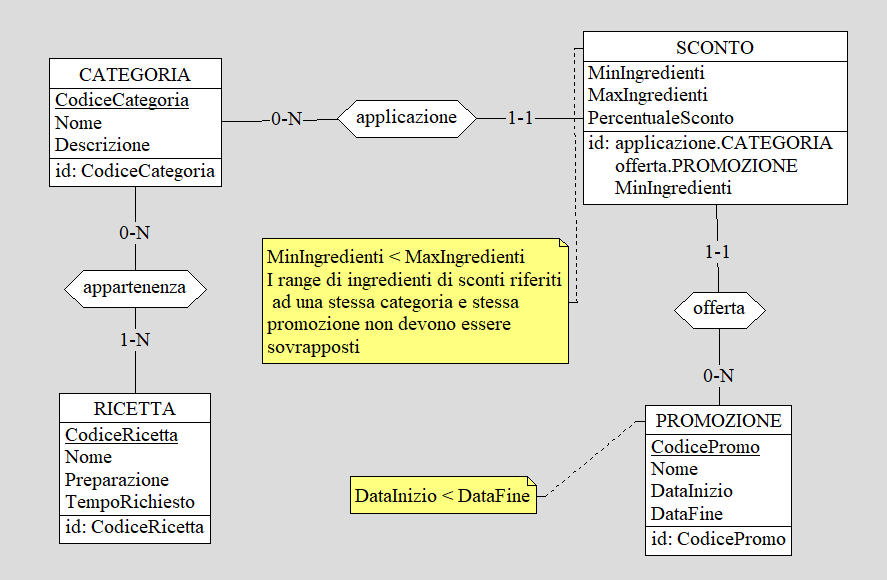
\includegraphics[width=1\textwidth]{images/conc_sconto.png}
    \caption{Schema scheletro per sconti e promozioni.}
    \label{fig:sconto} % Etichetta per fare riferimento: vedi Figura \ref{fig:mia_immagine}
\end{figure}

La \textbf{promozione} è stata modellata come semplice entità, con codice promozionale e range di date per rendere la promo periodica.
Osservando il dominio si è individuata la dipendenza

\textbf{Promozione, Categoria, Range Ingredienti -> Sconto}

E' stato quindi necessario reificare lo \textbf{sconto} in un’entità apposita, identificata dagli attributi/entità da cui essa dipende.\\
Per quanto riguarda il range del numero di ingredienti si è deciso di considerare solo “MinIngredienti” come identificatore, evidenziando i vincoli inespressi come si può notare in figura.

L’associazione \textbf{applicazione} è del tipo 1 a N in quanto uno \textbf{sconto} si riferisce ad una specifica \textbf{categoria}, mentre una \textbf{categoria} può avere più possibili \textbf{sconti} (ad esempio per promozioni e/o range di ingredienti diversi).\\
Infine l’associazione \textbf{offerta} è anch’essa di tipo 1 a N, per ragionamento analogo.


\section{Amministratore}

Nel panorama analizzato si suppone che l’amministratore sia uno solo e che egli sia solamente responsabile di popolare parte del database ed eventualmente di aggiornare i suoi dettagli; per fare ciò non è necessario memorizzare alcun suo dato.
Di conseguenza si è deciso di non tenerne conto nello schema E/R completo.

Si noti che nello schema concettuale finale viene aggiunto un ulteriore attributo “Ruolo” in UTENTE, al solo fine di distinguere gli utenti standard dagli amministratori al momento del login al sito.


\section{Schema concettuale finale}

Per la produzione dello schema concettuale finale si sono utilizzati e uniti gli schemi E/R relativi ai sottoproblemi precedentemente illustrati.

Come ultima modifica allo schema finale si è deciso di inserire due ulteriori attributi booleani:
\begin{itemize}
    \item “Attivo” in UTENTE
    \item “Rimossa” in RICETTA
\end{itemize}
Questi attributi sono stati aggiunti al fine di poter implementare facilmente l’operazione A6 di rimozione utenti.

La scelta di utilizzare una cancellazione logica (tramite attributo booleano) anziché una cancellazione fisica del record è motivata dal fatto che sia UTENTE che RICETTA sono coinvolti in numerose relazioni con altre entità (ORDINE, acquisto, recensione, composizione, ecc.), che nel tempo accumulano un volume rilevante di istanze storiche. \\
Una cancellazione fisica dell'utente o della ricetta comporterebbe la perdita — o la necessità di cancellazione a cascata — di tutti i dati storici ad essi collegati (ordini effettuati, recensioni scritte, ricette pubblicate), compromettendo l'integrità referenziale e la consultabilità dello storico anche da parte di altri utenti non coinvolti nella rimozione.

L'introduzione degli attributi "Attivo" e "Rimossa" consente quindi di:
\begin{itemize}
    \item mantenere l'integrità e la coerenza dei dati storici legati a ordini e recensioni già effettuati;
    \item impedire che un utente rimosso possa autenticarsi o effettuare nuove operazioni (pubblicare ricette, effettuare ordini, scrivere recensioni);
    \item impedire che una ricetta "rimossa" venga mostrata o resa acquistabile ai fini di nuove operazioni, pur restando visibile negli storici già esistenti;
    \item semplificare l'operazione A6, che si riduce a un semplice aggiornamento del valore dell'attributo, evitando la gestione più complessa di eliminazioni a cascata sulle relazioni coinvolte.
\end{itemize}

\begin{figure}[H]
    \centering
    % Regola la larghezza. 0.8\textwidth significa "80% della larghezza del testo".
    % Puoi usare anche cm, es: width=10cm
    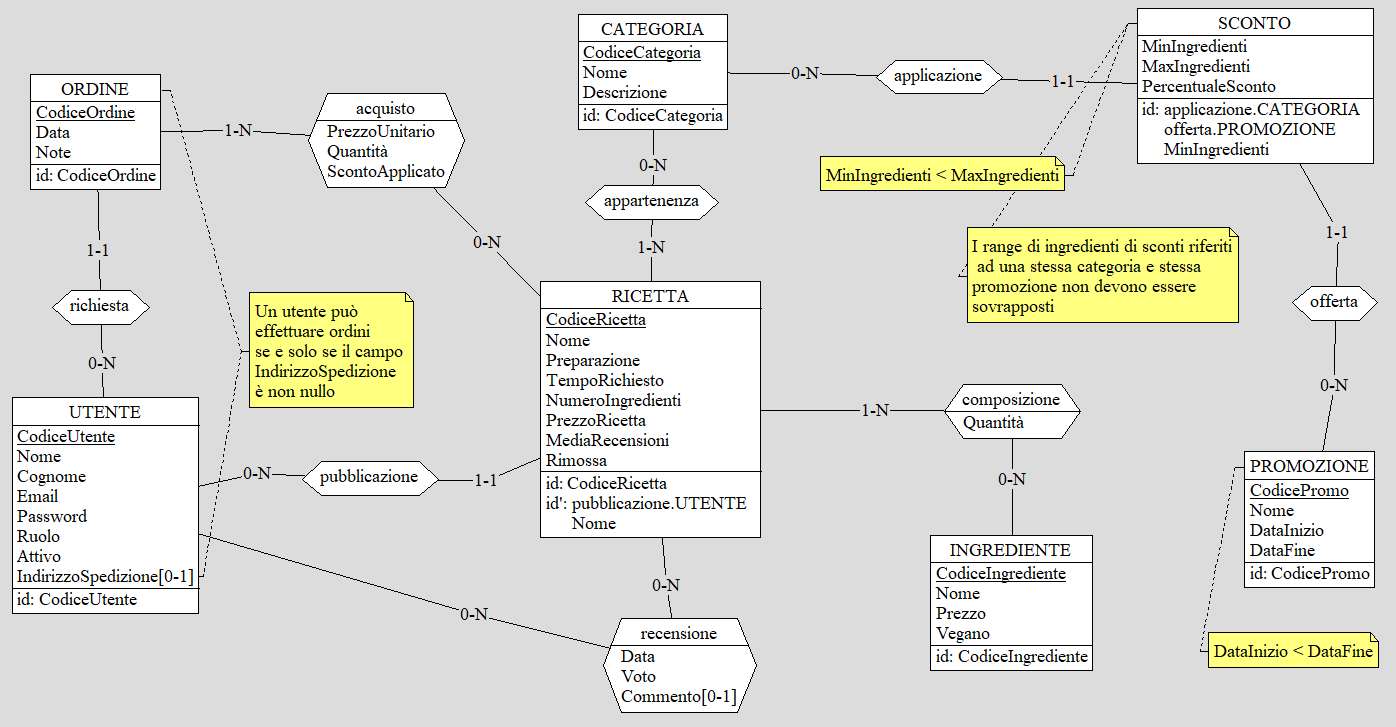
\includegraphics[width=1\textwidth]{images/conc_finale.png}
    \caption{Schema E/R completo.}
    \label{fig:conc_fin} % Etichetta per fare riferimento: vedi Figura \ref{fig:mia_immagine}
\end{figure}